%!TEX program = xelatex
\documentclass{article}
\usepackage{amsthm,amsmath,amssymb}
\usepackage[UTF8]{ctex}
\usepackage[tc]{titlepic}
\usepackage{titlesec}
\usepackage{cite}
\usepackage{fancyhdr}
\usepackage{booktabs}
\usepackage{graphicx}
\usepackage{subfigure}
\usepackage{float}
\usepackage{geometry}
\usepackage[section]{placeins}
\usepackage{makeidx}
\usepackage{mathrsfs}
\usepackage{color}
\usepackage{ulem}
\usepackage{enumitem}
\geometry{a4paper,scale=0.8}
\pagestyle{fancy}

\usepackage{hyperref}
\hypersetup{hypertex=true, colorlinks=true, linkcolor=blue, anchorcolor=blue, citecolor=blue}

\usepackage{listings}
\lstset{
    language=Python,
    basicstyle=\small\ttfamily,
    keywordstyle=\color{blue},
    commentstyle=\color{green},
    stringstyle=\color{red},
    showstringspaces=false,
    breaklines=true,
}

\lhead{第 1 次作业\\\today}
\chead{中国科学技术大学\\	DS4001 人工智能原理与技术}

\rhead{Homework 1\\ {\CTEXoptions[today=old]\today}}
\newcommand{\upcite}[1]{\textsuperscript{\cite{#1}}}

\titleformat*{\section}{\bfseries\Large}
\titleformat*{\subsection}{\bfseries\large}

\title{\bfseries 第一次作业(搜索问题)}
\author{高茂航  \quad  PB22061161}

\begin{document}
\maketitle
\textcolor{red}{\textbf{本次作业需独立完成,不允许任何形式的抄袭行为,如被发现会有相应惩罚。在上方修改你的姓名学号,说明你同意本规定。}}
% \clearpage

\section*{问题0:引入(30 分)}
\subsection*{1.最短路径问题(12分)}
\subsubsection*{a.回答问题(2分)}
$\mathcal{D}_1 \circ d_{v_1}(v_2)=d_{v_1}(v_2)=10$
\subsubsection*{b.证明(2分)}
若$\mathcal{D}_k \circ d_{s}(v_k)=min_{v \in V-\{v_0,...v_{k-1}\}}\{d_s(v)+w_{vv_k}\}\neq d_s(v_k)=min_{v\in V}\{d_s(v)+w_{vv_k}\}$,

则$\exists h \in \{v_{k+1},v_{k+2},...,v_{n}\}$,使得$\mathcal{D}_k \circ d(v_k)=d_s(h)\leqslant d_s(v_k)$,即h是到s第k近点,与假设矛盾。

\subsubsection*{c.证明(4分)}
$k=0$时显然成立。

设$k-1$时成立,即$\mathcal{D}_{k-1} \circ d(v_{k-1})\leqslant min_{v \in V-\{v_0,...v_{k-2}\}}d(v)$,

假如$\mathcal{D}_{k} \circ d(v_k)> min_{v \in V-\{v_0,...v_{k-1}\}}d(v)$,
则$\exists h,j \in \{v_{0},v_{1},...,v_{k-1}\}$,并在$d_s(h)+d_h(v_k)>d_s(j)+d_j(v_k)$时将$d_s(v_k)$更新为$d_s(h)+d_h(v_k)$,与假设矛盾。

\subsubsection*{d.回答问题(2分)}
$\mathcal{D}_{k}$表示选取$min_{v \in V-\{v_0,...v_{k-1}\}}d(v)$对应的点作为$v_k$,并用$v_k$更新$d(v),v\in V-\{v_0,...v_{k}\}$。
算符每作用一次就将未求得最短路径的点集减少一个,直到所有点都求得最短路径。
该算符的本质思想是使$d(v)$逐渐减小到$d_s(v)$。
\subsubsection*{e.证明(2分)}

若$d_s(u)\neq min_{v \in V}\{d_s(v)+w_{vu}\}$,

则设$d_s(u)=l_s(v)+w_{vu}$,其中$l_s(v)$是s到v的一条非最短路径,

又因为$l_s(v)+w_{vu}>d_s(v)+w_{vu}$,所以$l_s(v)+w_{vu}$不是s到u的最短路径,与假设矛盾。
$\exists v_1 \in V$,使得$d_s(u)=d_s(v_1)+w_{v_1u}>min_{v \in V}\{d_s(v)+w_{vu}\}=d_1$,
即$d_s(u)$不是最短路径长度,与假设矛盾。

\subsection*{2.A*算法,判断对错并说明原因(10分)}

\begin{enumerate}
    \item[a] 正确,因为Dijkstra算法就是不考虑启发函数下的$A^*$算法。
    \item[b] 正确,因为h(u)可能会影响要选择哪一个点,进而影响d(u)的更新。
    \item[c] 错误,因为d(u)都是基于各点之间的距离来更新的,因此即使用了h(u)也不存在某个d(u)不是某条路径长度的情况。
    \item[d] 正确,使用优先队列(通常是二叉堆)取每个节点的时间复杂度是$O(logn)$,所以总时间复杂度是$O(nlogn)$,对所有节点则为$O(nlogn)$,边数为m,所以总时间复杂度是$O(nlogn+m)$。
    \item[e] 正确,因为若$d_s(u) + h(u)\leqslant  d_s(v) + h(v)\rightarrow d_s(u)\leqslant  d_s(v)$,则h(u)对选点的判断没有影响,即选点顺序和Dijikstra算法一样。
\end{enumerate}

\subsection*{3.网格城市(8 分)}

\subsection*{a.回答问题(8分)}

$m \geqslant 0$时,最低成本路线唯一,即先y轴从原点走到(0,n),再从(0,n)走到(m,n),最低成本为$\lvert n \rvert+m+\frac{(1+m)m}{2}=\lvert n \rvert+\frac{(3+m)m}{2}$。

$m < 0$时,最低成本路线不唯一,只需做到总步数为$\lvert n \rvert+\lvert m \rvert$即可,最低成本为$\lvert n \rvert+\lvert m \rvert$。
\section*{问题1:查找最短路径(12分)}
\subsection*{a.代码实现ShortestPathProblem部分(8分)}
\begin{lstlisting}
class ShortestPathProblem(SearchProblem):
    """The illustration and __init___ part is ommited here."""

    def startState(self) -> State:
        # BEGIN_YOUR_CODE (our solution is 1 line of code, but don't worry if you deviate from this)
        return State(location=self.startLocation, memory=None)
        # END_YOUR_CODE

    def isEnd(self, state: State) -> bool:
        # BEGIN_YOUR_CODE (our solution is 1 line of code, but don't worry if you deviate from this)
        return self.endTag in self.cityMap.tags[state.location]
        # END_YOUR_CODE

    def successorsAndCosts(self, state: State) -> List[Tuple[str, State, float]]:
        # BEGIN_YOUR_CODE (our solution is 7 lines of code, but don't worry if you deviate from this)
        successors = []
        for neighbor, cost in self.cityMap.distances[state.location].items():
            new_state = State(location=neighbor, memory=None)
            successors.append((neighbor, new_state, cost))
        return successors
        # END_YOUR_CODE
\end{lstlisting}

\subsection*{b.路线可视化(4分)}
\subsubsection*{1.比较有趣的路线}
\begin{lstlisting}
startLocation = "8763079035"
endTag = "label=6107399985"
\end{lstlisting}
\begin{figure}[H]
	\centering 
	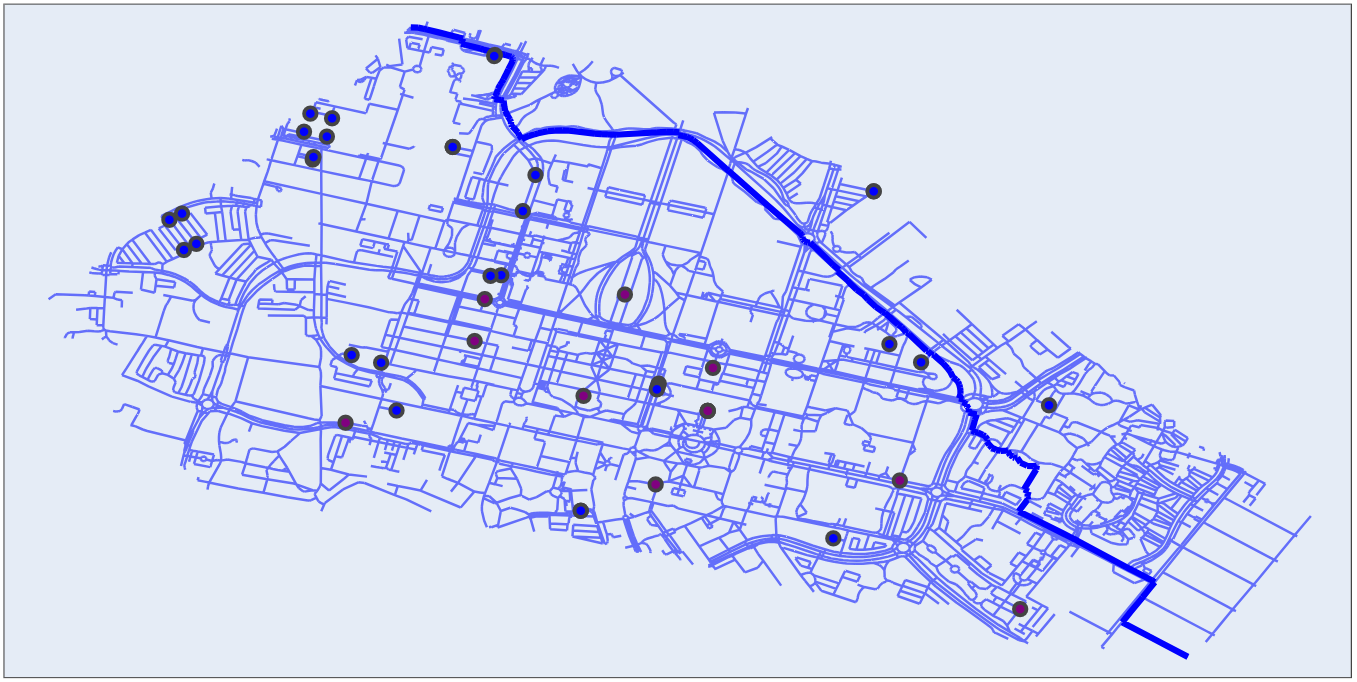
\includegraphics[height=6cm,width=14cm]{1.png}
    \caption{比较有趣的路线}
\end{figure}
这条路线从校园的西北角穿到东南角,经过的地点比较多。
\subsubsection*{2.比较短而无聊的路线}
    \begin{lstlisting}
startLocation = "8763079035"
endTag = "entrance=yes"
    \end{lstlisting}
	
	\begin{figure}[H]
		\centering 
		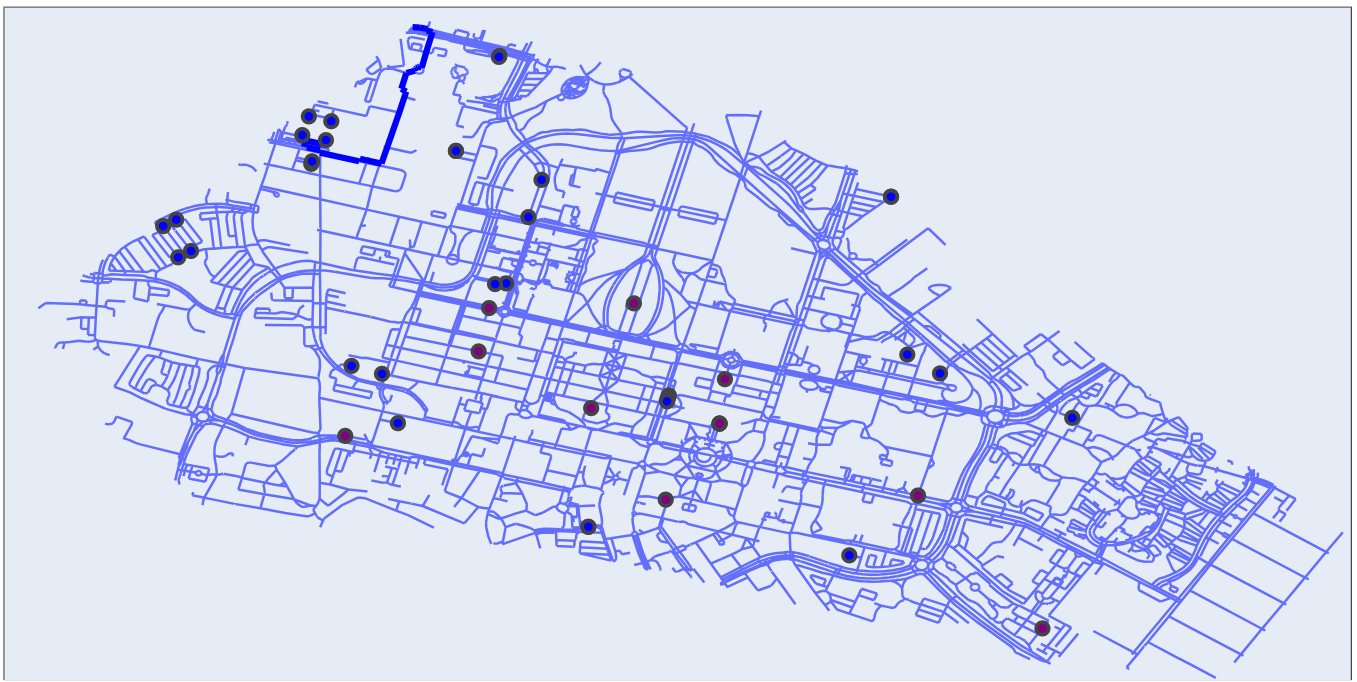
\includegraphics[height=6cm,width=14cm]{3.png}
        \caption{比较短而无聊的路线}
    \end{figure}
这条路线从校园西北角通到有入口的地方,比较短,但确实符合要求,如果我希望去更远处的入口,应该换一个更特别的标签来建模。

\section*{问题2:查找带无序途径点的最短路径(20分)}
\subsection*{a.代码实现WaypointsShortestPathProblem部分(12分)}
 
 \begin{lstlisting}
class WaypointsShortestPathProblem(SearchProblem):
    """The illustration and __init___ part is ommited here."""

    def startState(self) -> State:
        # BEGIN_YOUR_CODE (our solution is 1 line of code, but don't worry if you deviate from this)
        return State(location=self.startLocation, memory=frozenset())
        # END_YOUR_CODE

    def isEnd(self, state: State) -> bool:
        # BEGIN_YOUR_CODE (our solution is 5 lines of code, but don't worry if you deviate from this)
        return self.endTag in self.cityMap.tags[state.location] and all(tag in state.memory for tag in self.waypointTags)
        # END_YOUR_CODE

    def successorsAndCosts(self, state: State) -> List[Tuple[str, State, float]]:
        # BEGIN_YOUR_CODE (our solution is 17 lines of code, but don't worry if you deviate from this)
        successors = []
        for nextLocation, distance in self.cityMap.distances[state.location].items():
            memory = set(state.memory)
            for tag in self.cityMap.tags[state.location]:
                if tag in self.waypointTags:
                    memory.add(tag)
        
            new_state = State(location=nextLocation, memory=frozenset(memory))
            successors.append((nextLocation,new_state,distance))
        return successors
        # END_YOUR_CODE
\end{lstlisting}

\subsection*{b.回答问题(4分)}
$n2^{k}$,k个标签的集合有$2^{k}$种可能状态,当每个点都遍历所有可能状态时即UCS可访问的最大状态数。

\subsection*{c.可视化(4分)}
\begin{lstlisting}
    startLocation = "8763079035"
    endTag = "label=6107399985"
    \end{lstlisting}
\begin{figure}[H]
    \centering 
    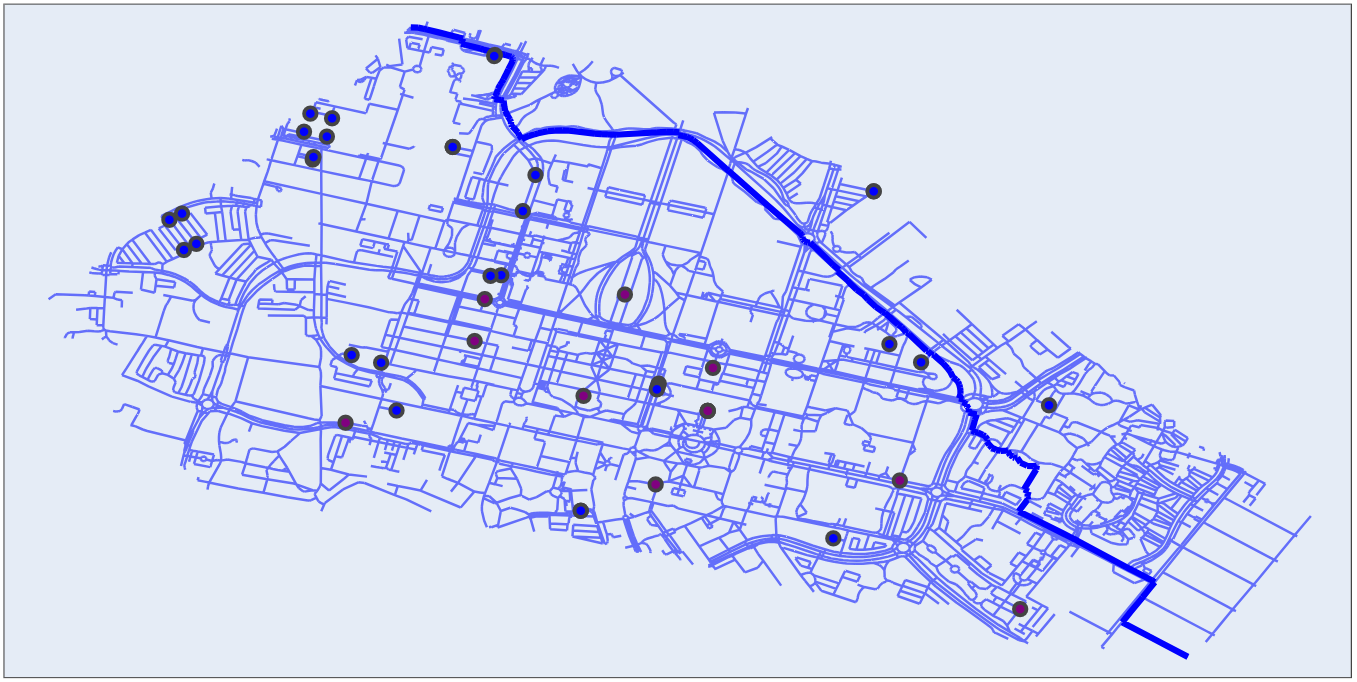
\includegraphics[height=6cm,width=14cm]{1.png}
    \caption{1b中第一条路线}
    \end{figure}
\begin{lstlisting}
waypointTags = ["crossing=uncontrolled", "bicycle=yes", "foot=yes", "kerb=lowered", "traffic_sign=stop"]
\end{lstlisting}
\begin{figure}[H]
	\centering 
	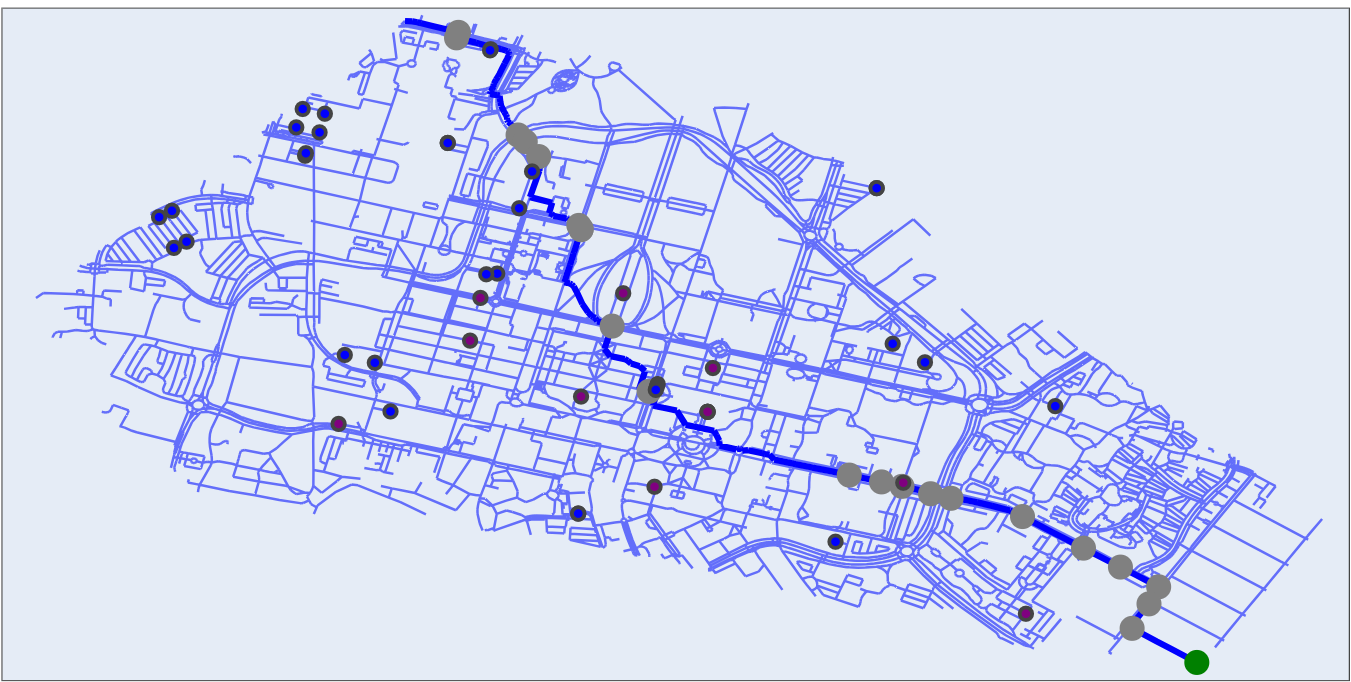
\includegraphics[height=6cm,width=14cm]{2.png}
    \caption{1b中第一条路线加了途径点后的结果}
	\end{figure}
    这张图的路径经过了指定的途径点,使得路径比1b的更长,但能去到更多地方。
\section*{问题3:使用 A*算法加快搜索速度(28分)}
\subsection*{a.代码实现aStarReduction的NewSearchProblem部分(8分)}

\begin{lstlisting}
def aStarReduction(problem: SearchProblem, heuristic: Heuristic) -> SearchProblem:
    class NewSearchProblem(SearchProblem):
        def startState(self) -> State:
            # BEGIN_YOUR_CODE (our solution is 1 line of code, but don't worry if you deviate from this)
            return problem.startState()
            # END_YOUR_CODE

        def isEnd(self, state: State) -> bool:
            # BEGIN_YOUR_CODE (our solution is 1 line of code, but don't worry if you deviate from this)
            return problem.isEnd(state)
            # END_YOUR_CODE

        def successorsAndCosts(self, state: State) -> List[Tuple[str, State, float]]:
            # BEGIN_YOUR_CODE (our solution is 8 lines of code, but don't worry if you deviate from this)
            successors = []
            for action, nextState, cost in problem.successorsAndCosts(state):
                newCost = cost + heuristic.evaluate(nextState) - heuristic.evaluate(state)
                successors.append((action, nextState, newCost))
            return successors
            # END_YOUR_CODE

    return NewSearchProblem()
\end{lstlisting}

\subsection*{b.代码实现StraightLineHeuristic部分(8分)}

\begin{lstlisting}
class StraightLineHeuristic(Heuristic):

    def __init__(self, endTag: str, cityMap: CityMap):
        self.endTag = endTag
        self.cityMap = cityMap
        # Precompute
        # BEGIN_YOUR_CODE (our solution is 5 lines of code, but don't worry if you deviate from this)
        self.end_locations = []
        for location, tags in self.cityMap.tags.items():
            if self.endTag in tags:
                self.end_locations.append(location)
        # END_YOUR_CODE

    def evaluate(self, state: State) -> float:
        # BEGIN_YOUR_CODE (our solution is 6 lines of code, but don't worry if you deviate from this)
        distances = []
        for end_location in self.end_locations:
            distance = computeDistance(self.cityMap.geoLocations[state.location], self.cityMap.geoLocations[end_location])
            distances.append(distance)
        return min(distances) if distances else 0
        # END_YOUR_CODE
\end{lstlisting}

\subsection*{c.代码实现NoWaypointsHeuristic部分(12分)}
\begin{lstlisting}
class NoWaypointsHeuristic(Heuristic):
    
    def __init__(self, endTag: str, cityMap: CityMap):
        # Precompute
        # BEGIN_YOUR_CODE (our solution is 25 lines of code, but don't worry if you deviate from this)
        self.endTag = endTag
        self.cityMap = cityMap
        self.locations = list(self.cityMap.geoLocations.keys())
        self.end_locations = [location for location, tags in self.cityMap.tags.items() if self.endTag in tags]
        self.shortest_paths = {}
        for location1 in self.end_locations:
            problem = ShortestPathProblem(location1, "label=0", cityMap)
            ucs = UniformCostSearch()
            ucs.solve(problem)
            for location2, cost in ucs.pastCosts.items():
                self.shortest_paths[(location2, location1)] = cost
        # END_YOUR_CODE

    def evaluate(self, state: State) -> float:
        # BEGIN_YOUR_CODE (our solution is 1 line of code, but don't worry if you deviate from this)
        distances = [self.shortest_paths[(state.location, end_location)] for end_location in self.end_locations]
        return min(distances) if distances else 0
        # END_YOUR_CODE
\end{lstlisting}


\section*{反馈(10分)}

\begin{itemize}
    \item 这次作业花了几天的空闲时间,主要用于看代码和思考3c。看代码的过程感觉比较困难,可能是因为内容比较多,但看明白后做得就很快了。3c的想法过于巧妙,很难想到;
    \item 感觉上课时讲得比较快,不太好消化,课后还要自己学很久,而且自己对相关代码也不够熟练。
\end{itemize}

\end{document}